%%%%%%%%%%%%%%%%%%%%%%%%%%%%%%%%%%%%%%%%%
%
% Using Diaz essay LaTeX template from:
% http://www.LaTeXTemplates.com
%
% Authors:
% Vel (vel@LaTeXTemplates.com)
% Nicolas Diaz (nsdiaz@uc.cl)
%
% License:
% CC BY-NC-SA 3.0 (http://creativecommons.org/licenses/by-nc-sa/3.0/)
%
%%%%%%%%%%%%%%%%%%%%%%%%%%%%%%%%%%%%%%%%%

% PACKAGES AND OTHER DOCUMENT CONFIGURATIONS
\documentclass[11pt]{diazessay} % Font size (can be 10pt, 11pt or 12pt)

\usepackage{listings}
\usepackage{tikz}
\usetikzlibrary{positioning}
\usetikzlibrary{arrows}

\lstset{frame=tb,
  language=C,
  aboveskip=3mm,
  belowskip=3mm,
  showstringspaces=false,
  columns=flexible,
  basicstyle={\small\ttfamily},
  numbers=none,
  numberstyle=\tiny\color{gray},
  keywordstyle=\color{blue},
  commentstyle=\color{black},
  %stringstyle=\color{mauve},
  breaklines=false,
  breakatwhitespace=false,
  tabsize=3
}

% Defines a `datastore' shape for use in DFDs.  This inherits from a
% rectangle and only draws two horizontal lines.
\makeatletter
\pgfdeclareshape{datastore}{
  \inheritsavedanchors[from=rectangle]
  \inheritanchorborder[from=rectangle]
  \inheritanchor[from=rectangle]{center}
  \inheritanchor[from=rectangle]{base}
  \inheritanchor[from=rectangle]{north}
  \inheritanchor[from=rectangle]{north east}
  \inheritanchor[from=rectangle]{east}
  \inheritanchor[from=rectangle]{south east}
  \inheritanchor[from=rectangle]{south}
  \inheritanchor[from=rectangle]{south west}
  \inheritanchor[from=rectangle]{west}
  \inheritanchor[from=rectangle]{north west}
  \backgroundpath{
    %  store lower right in xa/ya and upper right in xb/yb
    \southwest \pgf@xa=\pgf@x \pgf@ya=\pgf@y
    \northeast \pgf@xb=\pgf@x \pgf@yb=\pgf@y
    \pgfpathmoveto{\pgfpoint{\pgf@xa}{\pgf@ya}}
    \pgfpathlineto{\pgfpoint{\pgf@xb}{\pgf@ya}}
    \pgfpathmoveto{\pgfpoint{\pgf@xa}{\pgf@yb}}
    \pgfpathlineto{\pgfpoint{\pgf@xb}{\pgf@yb}}
 }
}
\makeatother

% TITLE SECTION
\title{\textbf{Diving into Linux Perf Ring Buffer}}
\author{\textbf{Leo Yan} \textit{<leo.yan@linaro.org>}} % Author and institution
\date{\today} % Date, use \date{} for no date

\def\code#1{\texttt{#1}}

%----------------------------------------------------------------------------------------

\begin{document}

\maketitle % Print the title section

% ABSTRACT AND KEYWORDS

\begin{abstract}
Linux perf ring buffer is not only used to transfer the PMU event data, it's also a fundamental mechanism for hardware tracing with Intel PT, Arm CoreSight, etc.  Therefore, the ring buffer implementation is critical and very challenge, it is required to provide high throughput, and should avoid causing any significant overload by itself for the buffer's management.

The purpose of this article is to provide a material if anyone wants to understand the internal of pref ring buffer. By diving into the details, it explains the perf ring buffer implementation and how the ring buffer is applicated in practice.
\end{abstract}

\hspace*{3.6mm}\textit{Keywords:} Linux, perf, ring buffer, throughput, profiling % Keywords
\vspace{30pt} % Vertical whitespace between the abstract and first section

% ESSAY BODY

\section*{Introduction}

Perf tool is a main stream profiling tool which is widely used in Linux community.  At the early time, it was originally designed to support CPU PMU events, like CPU cycles, cache access and misses events, etc; afterwards, it was extended to support timers, software events (E.g. Ftrace tracepoints).  Nowdays, it has integrated with the hardware trace and even can co-work with eBPF tracing.

To support these kind events, especially if developers want to record multiple events in one go, the ring buffer plays a critical role for event recording, the kernel and perf tool in the user space use the ring buffer to exchange data, and at the end stores record into data file.

The throughput is a big challenge in the implementation, particularly, from the performance pespective, it would be very interesting to know how the buffer is synchronized between user space and kernel, and how to support SMP if the buffer is shared by multiple CPUs.  This article tries to dive into these details and give out answers to cate our curiosity.

In the sequential sections, the content is arranged as:
\begin{itemize}
	\item The introduction for basic algorithm of the ring buffer;
	\item The mechanim for AUX ring buffer;
	\item At last, using Arm CoreSight as an example to explain how the ring buffer works with hardware trace.
\end{itemize}

\section*{Implementation for the ring buffer}

\subsection*{Basic algorithm}

As said in the textbook, the ring buffer should be managed by a head pointer and a tail pointer; the head pointer is manipulated by a writer and the tail pointer is updated by a reader respectively.

\begin{center}
\par
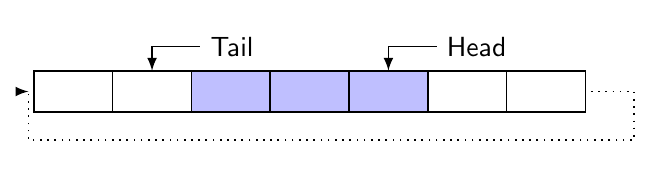
\begin{tikzpicture}[>=latex,font=\sffamily,semithick,scale=1.75]
	\centering
	\node [minimum width=1cm,minimum height=1.5em,outer sep=0pt,draw=black,fill=white] at (0,0) (A) {};
        \node [minimum width=1cm,minimum height=1.5em,outer sep=0pt,draw=black,fill=white,anchor=west] at (A.east) (B) {};
        \node [minimum width=1cm,minimum height=1.5em,outer sep=0pt,draw=black,fill=blue!25,anchor=west] at (B.east) (C) {};
        \node [minimum width=1cm,minimum height=1.5em,outer sep=0pt,draw=black,fill=blue!25,anchor=west] at (C.east) (D) {};
        \node [minimum width=1cm,minimum height=1.5em,outer sep=0pt,draw=black,fill=blue!25,anchor=west] at (D.east) (E) {};
        \node [minimum width=1cm,minimum height=1.5em,outer sep=0pt,draw=black,fill=white,anchor=west] at (E.east) (F) {};
        \node [minimum width=1cm,minimum height=1.5em,outer sep=0pt,draw=black,fill=white,anchor=west] at (F.east) (G) {};
	\draw [->,shorten >=2pt,shorten <=2pt,semithick,dotted] (G.east) -- +(1em,0em) -- +(1em,-1em) -- +(-11.5em,-1em) -- +(-11.5em,0em) -- (A.west);
	\draw [<-] (E.north) -- +(0em,.5em) -- +(1em,.5em) node [right] (Head) {Head};
	\draw [<-] (B.north) -- +(0em,.5em) -- +(1em,.5em) node [right] (Tail) {Tail};
\end{tikzpicture}

\bigskip

\par
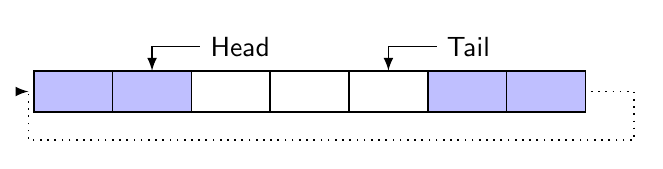
\begin{tikzpicture}[>=latex,font=\sffamily,semithick,scale=1.75]
	\node [minimum width=1cm,minimum height=1.5em,outer sep=0pt,draw=black,fill=blue!25] at (0,0) (A) {};
        \node [minimum width=1cm,minimum height=1.5em,outer sep=0pt,draw=black,fill=blue!25,anchor=west] at (A.east) (B) {};
        \node [minimum width=1cm,minimum height=1.5em,outer sep=0pt,draw=black,fill=white,anchor=west] at (B.east) (C) {};
        \node [minimum width=1cm,minimum height=1.5em,outer sep=0pt,draw=black,fill=white,anchor=west] at (C.east) (D) {};
        \node [minimum width=1cm,minimum height=1.5em,outer sep=0pt,draw=black,fill=white,anchor=west] at (D.east) (E) {};
        \node [minimum width=1cm,minimum height=1.5em,outer sep=0pt,draw=black,fill=blue!25,anchor=west] at (E.east) (F) {};
        \node [minimum width=1cm,minimum height=1.5em,outer sep=0pt,draw=black,fill=blue!25,anchor=west] at (F.east) (G) {};
	\draw [->,shorten >=2pt,shorten <=2pt,semithick,dotted] (G.east) -- +(1em,0em) -- +(1em,-1em) -- +(-11.5em,-1em) -- +(-11.5em,0em) -- (A.west);
	\draw [<-] (E.north) -- +(0em,.5em) -- +(1em,.5em) node [right] (Tail) {Tail};
	\draw [<-] (B.north) -- +(0em,.5em) -- +(1em,.5em) node [right] (Head) {Head};
\end{tikzpicture}
\par
\textbf{Figure 1: Ring buffer (without and with overflow)}
\end{center}

Similarily, perf uses the same way to manage the ring buffer.  There have two actors: a page contains the control structure for ring buffer management, and the ring buffer; following the naming convention, the page containing the control structure is named as "user page".  The user page and the ring buffer are mapped to user space via the virtual mapping area (VMA) in the continuous address space, and the user page is mapped prior to the buffer.

The control structure is defined as \code{perf\_event\_mmap\_page} which contains the head pointer \code{data\_head} and the tail pointer \code{data\_tail}.  When the kernel starting to fill records into the ring buffer, it modifies the head pointer to reserve the memory so that later can safely store events into the buffer; on the other side, the perf tool updates the tail pointer when consumes data from the ring buffer.

\begin{center}
\par
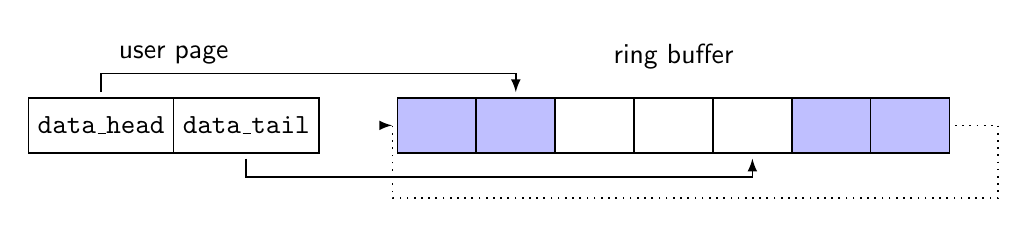
\begin{tikzpicture}[>=latex,font=\sffamily,semithick,scale=1.75]
	\node [minimum width=1cm,minimum height=2em,outer sep=0pt,draw=black,fill=white] at (0,0) (A) {\code{data\_head}};
	\node [minimum height=2em] at (A.east) (A2) {};
	\node [minimum width=1cm,minimum height=2em,outer sep=0pt,draw=black,fill=white,anchor=west] at (A.east) (B) {\code{data\_tail}};
        \node [minimum width=1cm,minimum height=2em,outer sep=0pt,draw=black,fill=blue!25,right=1cm of B] (C) {};
        \node [minimum width=1cm,minimum height=2em,outer sep=0pt,draw=black,fill=blue!25,anchor=west] at (C.east) (D) {};
        \node [minimum width=1cm,minimum height=2em,outer sep=0pt,draw=black,fill=white,anchor=west] at (D.east) (E) {};
        \node [minimum width=1cm,minimum height=2em,outer sep=0pt,draw=black,fill=white,anchor=west] at (E.east) (F) {};
        \node [minimum width=1cm,minimum height=2em,outer sep=0pt,draw=black,fill=white,anchor=west] at (F.east) (G) {};
        \node [minimum width=1cm,minimum height=2em,outer sep=0pt,draw=black,fill=blue!25,anchor=west] at (G.east) (H) {};
        \node [minimum width=1cm,minimum height=2em,outer sep=0pt,draw=black,fill=blue!25,anchor=west] at (H.east) (I) {};
	\node [minimum width=1cm,minimum height=2em,outer sep=0pt,above=0.5em of A2] (control) {user page};
	\node [minimum width=1cm,minimum height=2em,outer sep=0pt,above=0.5em of F] (buffer) {ring buffer};
	\draw [->,shorten >=2pt,shorten <=2pt,semithick,dotted] (I.east) -- +(1em,0em) -- +(1em,-1.5em) -- +(-11.5em,-1.5em) -- +(-11.5em,0em) -- (C.west);
	\draw [->,shorten >=2pt,shorten <=2pt,semithick] (A.north) -- +(0em,.5em) -| (D.north);
	\draw [->,shorten >=2pt,shorten <=2pt,semithick] (B.south) -- +(0em,-.5em) -| (G.south);
\end{tikzpicture}
\par
\textbf{Figure 2: Perf ring buffer}
\end{center}

Though the kernel allocates at once for all memory pages, including a dedicated page for the user page and the sequential pages for ring buffer, it's deferred to map the the pages to VMA area until the perf tool accesses the buffer from the user space.  In other words, the kernel event subsystem uses the linear kernel virtual address for accessing the ring buffer, the perf tool in the user space accesses the ring buffer via VMA, and at the first time accesses the buffer's page, a data abort exeception for page fault is taken and the kernel uses this occasion to map the page into VMA, thus the perf tool can continue to access the page after return back from page fault.

The function \code{perf\_mmap\_fault()} is invoked for handling page fault, which uses the function \code{perf\_mmap\_to\_page()} to figure out which page should be mapped. If \code{pg\_off} is zero it returns the pointer for the ring buffer's user page, otherwise it finds out the ring buffer's data page by using \code{pg\_off-1} as the page index (since the first page in VMA is reserved for user page, it produces offset '1' between the VMA index and data pages index).

\begin{lstlisting}
static vm_fault_t perf_mmap_fault(struct vm_fault *vmf)
{
        struct perf_event *event = vmf->vma->vm_file->private_data;
        struct perf_buffer *rb;
        vm_fault_t ret = VM_FAULT_SIGBUS;

        if (vmf->flags & FAULT_FLAG_MKWRITE) {
                if (vmf->pgoff == 0)
                        ret = 0;
                return ret;
        }

        rcu_read_lock();
        rb = rcu_dereference(event->rb);
        if (!rb)
                goto unlock;

        if (vmf->pgoff && (vmf->flags & FAULT_FLAG_WRITE))
                goto unlock;

        vmf->page = perf_mmap_to_page(rb, vmf->pgoff);
        if (!vmf->page)
                goto unlock;

        get_page(vmf->page);
        vmf->page->mapping = vmf->vma->vm_file->f_mapping;
        vmf->page->index   = vmf->pgoff;

        ret = 0;
unlock:
        rcu_read_unlock();

        return ret;
}
\end{lstlisting}

\subsection*{Ring buffer allocation for different modes}

Perf profiles programs with different modes: per thread mode, per cpu mode, and system wide mode; the question is how the ring buffer is organized for these modes. This section describes what's exactly these modes and how the ring buffer can meet the requirement for them; at last we can review if there have any race conditions for the ring buffer caused in these modes.

\subsubsection*{Per thread mode}

For the per-thread mode, by specifying option \code{----per--thread} in perf command, the ring buffer is allocated for every profiled thread.  In this mode when the profiled thread is scheduled on a CPU, the events on that CPU will be enabled; and if the thread is cheduled out from the CPU, the events on the CPU will be disabled.  And if the thread is migrated from one CPU to another CPU, the events will be disabled on the previous CPU and enabled on the next CPU correspondingly.

\begin{center}
\par
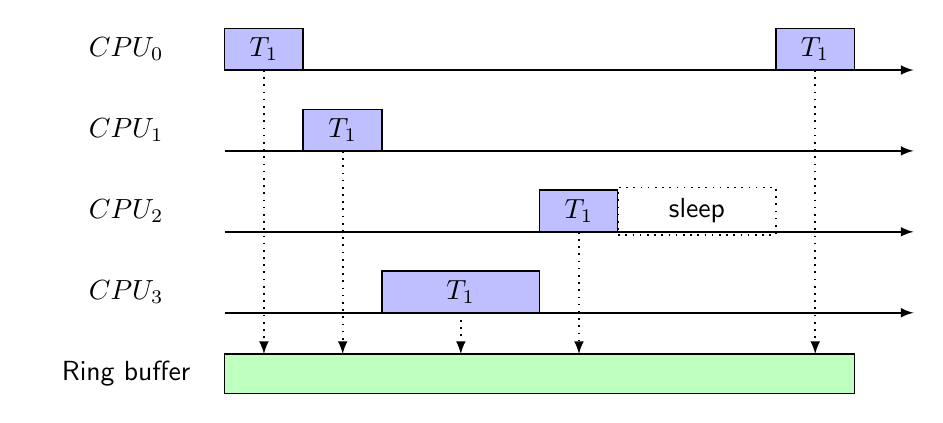
\begin{tikzpicture}[>=latex,font=\sffamily,semithick,scale=1.75]
	\node [minimum width=2.5cm,minimum height=.5cm,outer sep=0pt] at (0,0) (cpu0) {\( CPU_0 \)};
	\node [minimum width=1cm,minimum height=.5cm,outer sep=0pt,draw=black,fill=blue!25,right=0cm of cpu0] at (cpu0.east) (cpu0_p1_0) {\(T_{1}\)};
	\node [minimum width=1cm,minimum height=.5cm,outer sep=0pt,draw=black,fill=blue!25,right=7cm of cpu0] (cpu0_p1_1) {\(T_{1}\)};
	\draw[->] (cpu0.south east) -- +(5cm,0);

	\node [minimum width=2.5cm,minimum height=.5cm,outer sep=0pt,below=.5cm of cpu0] (cpu1) {\(CPU_{1}\)};
	\node [minimum width=1cm,minimum height=.5cm,outer sep=0pt,draw=black,fill=blue!25,right=1cm of cpu1] at (cpu1.east) (cpu1_p1_0) {\(T_{1}\)};
	\draw[->] (cpu1.south east) -- +(5cm,0);

	\node [minimum width=2.5cm,minimum height=.5cm,outer sep=0pt,below=.5cm of cpu1] (cpu2) {\(CPU_{2}\)};
	\node [minimum width=1cm,minimum height=.5cm,outer sep=0pt,draw=black,fill=blue!25,right=4cm of cpu2] (cpu2_p1_0) {\(T_{1}\)};
	\node [minimum width=2cm,minimum height=.6cm,outer sep=0pt,draw=black,fill=white,dotted,right=5cm of cpu2] (cpu2_p1_1) { sleep };
	\draw[->] (cpu2.south east) -- +(5cm,0);

	\node [minimum width=2.5cm,minimum height=.5cm,outer sep=0pt,below=.5cm of cpu2] (cpu3) {\(CPU_{3}\)};
	\node [minimum width=2cm,minimum height=.5cm,outer sep=0pt,draw=black,fill=blue!25,right=2cm of cpu3] (cpu3_p1_0) {\(T_{1}\)};
	\draw[->] (cpu3.south east) -- +(5cm,0);

	\node [minimum width=2.5cm,minimum height=.5cm,outer sep=0pt,below=.5cm of cpu3] (rb) {Ring buffer};
	\node [minimum width=8cm,minimum height=.5cm,outer sep=0pt,draw=black,fill=green!25,right=0cm of rb] (rb_0) {};

	\draw[->,dotted] (cpu0_p1_0.south) -- (cpu0_p1_0.south|-rb_0.north);
	\draw[->,dotted] (cpu1_p1_0.south) -- (cpu1_p1_0.south|-rb_0.north);
	\draw[->,dotted] (cpu2_p1_0.south) -- (cpu2_p1_0.south|-rb_0.north);
	\draw[->,dotted] (cpu3_p1_0.south) -- (cpu3_p1_0.south|-rb_0.north);
	\draw[->,dotted] (cpu0_p1_1.south) -- (cpu0_p1_1.south|-rb_0.north);
\end{tikzpicture}
\par
\textbf{Figure 3: Ring buffer for per-thread mode}
\end{center}

As shown in the figure 3, when perf runs in per-thread mode, a ring buffer is allocated for the profiled thread \(T_{1}\).  The ring buffer is dedicated for the thread \(T_{1}\), and no matter the thread is scheduled on which CPUs.  If the thread \(T_{1}\) is running, the perf events will be recorded into the ring buffer; during the thread's sleeping period, all associated events will be disabled, thus the ring buffer will not record any trace data.

\subsubsection*{Per CPU mode}

The option \code{--C} is used to collect samples only on the list of CPUs, the ring buffers are allocated for the specified CPUs.  For the example in figure 4, the perf command receives option \code{--C 0,2}, as the result, two ring buffers serve for CPU0 and CPU2 separately.

\begin{center}
\par
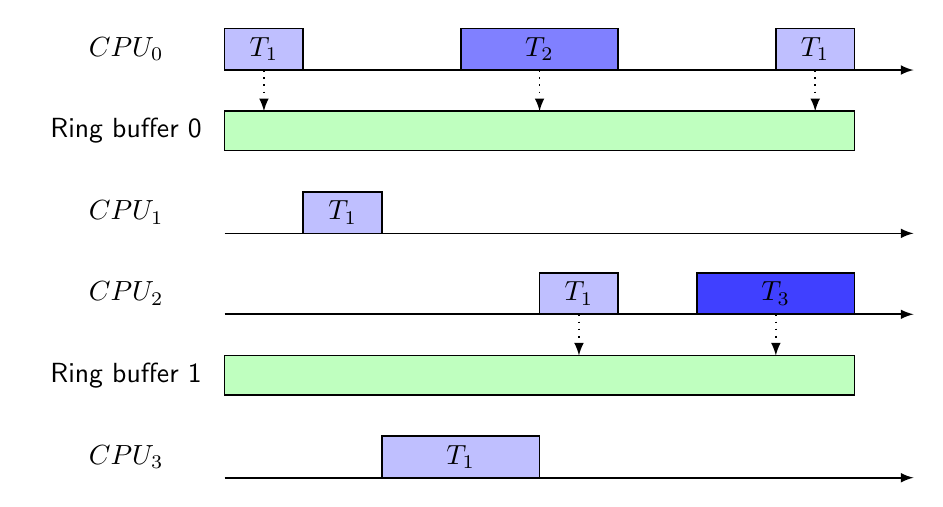
\begin{tikzpicture}[>=latex,font=\sffamily,semithick,scale=1.75]
	\node [minimum width=2.5cm,minimum height=.5cm,outer sep=0pt] at (0,0) (cpu0) {\( CPU_0 \)};
	\node [minimum width=1cm,minimum height=.5cm,outer sep=0pt,draw=black,fill=blue!25,right=0cm of cpu0] at (cpu0.east) (cpu0_p1_0) {\(T_{1}\)};
	\node [minimum width=2cm,minimum height=.5cm,outer sep=0pt,draw=black,fill=blue!50,right=3cm of cpu0] at (cpu0.east) (cpu0_p2_0) {\(T_{2}\)};
	\node [minimum width=1cm,minimum height=.5cm,outer sep=0pt,draw=black,fill=blue!25,right=7cm of cpu0] (cpu0_p1_1) {\(T_{1}\)};
	\draw[->] (cpu0.south east) -- +(5cm,0);

	\node [minimum width=2.5cm,minimum height=.5cm,outer sep=0pt,below=.5cm of cpu0] (rb0_txt) {Ring buffer 0};
	\node [minimum width=8cm,minimum height=.5cm,outer sep=0pt,draw=black,fill=green!25,right=0cm of rb0_txt] (rb0) {};

	\node [minimum width=2.5cm,minimum height=.5cm,outer sep=0pt,below=.5cm of rb0_txt] (cpu1) {\(CPU_{1}\)};
	\node [minimum width=1cm,minimum height=.5cm,outer sep=0pt,draw=black,fill=blue!25,right=1cm of cpu1] at (cpu1.east) (cpu1_p1_0) {\(T_{1}\)};
	\draw[->] (cpu1.south east) -- +(5cm,0);

	\node [minimum width=2.5cm,minimum height=.5cm,outer sep=0pt,below=.5cm of cpu1] (cpu2) {\(CPU_{2}\)};
	\node [minimum width=1cm,minimum height=.5cm,outer sep=0pt,draw=black,fill=blue!25,right=4cm of cpu2] (cpu2_p1_0) {\(T_{1}\)};
	\node [minimum width=2cm,minimum height=.5cm,outer sep=0pt,draw=black,fill=blue!75,right=6cm of cpu2] (cpu2_p3_0) {\(T_{3}\)};
	\draw[->] (cpu2.south east) -- +(5cm,0);

	\node [minimum width=2.5cm,minimum height=.5cm,outer sep=0pt,below=.5cm of cpu2] (rb1_txt) {Ring buffer 1};
	\node [minimum width=8cm,minimum height=.5cm,outer sep=0pt,draw=black,fill=green!25,right=0cm of rb1_txt] (rb1) {};

	\node [minimum width=2.5cm,minimum height=.5cm,outer sep=0pt,below=.5cm of rb1_txt] (cpu3) {\(CPU_{3}\)};
	\node [minimum width=2cm,minimum height=.5cm,outer sep=0pt,draw=black,fill=blue!25,right=2cm of cpu3] (cpu3_p1_0) {\(T_{1}\)};
	\draw[->] (cpu3.south east) -- +(5cm,0);


	\draw[->,dotted] (cpu0_p1_0.south) -- (cpu0_p1_0.south|-rb0.north);
	\draw[->,dotted] (cpu0_p1_1.south) -- (cpu0_p1_1.south|-rb0.north);
	\draw[->,dotted] (cpu0_p2_0.south) -- (cpu0_p2_0.south|-rb0.north);

	\draw[->,dotted] (cpu2_p1_0.south) -- (cpu2_p1_0.south|-rb1.north);
	\draw[->,dotted] (cpu2_p3_0.south) -- (cpu2_p3_0.south|-rb1.north);
\end{tikzpicture}
\par
\textbf{Figure 4: Ring buffer for per-cpu mode}
\end{center}

On the other hand, in this example even there have tasks running on CPU1 and CPU3, since the ring buffer is absent for these two CPUs, any activities on them will be ignored.

A usage case is to combine the options for per-thread mode and per-CPU mode, e.g. the option \code{--C 0,2 ----per--thread} is specified together; in this case, samples are recorded only when the profiled thread is scheduled on any of the listed CPUs.

\subsubsection*{System wide mode}

By default if without specifying mode, or explicitly using option \code{--a} or \code{----all--cpus}, perf collects samples on all CPUs, with the system wide mode.

In this mode, every CPU has its dedicated ring buffer; the interested events will be always enabled and sampled on every CPU, thus all threads are monitored, and the samples are recorded into the ring buffer belonging to the CPU which the events occurred on.

\begin{center}
\par
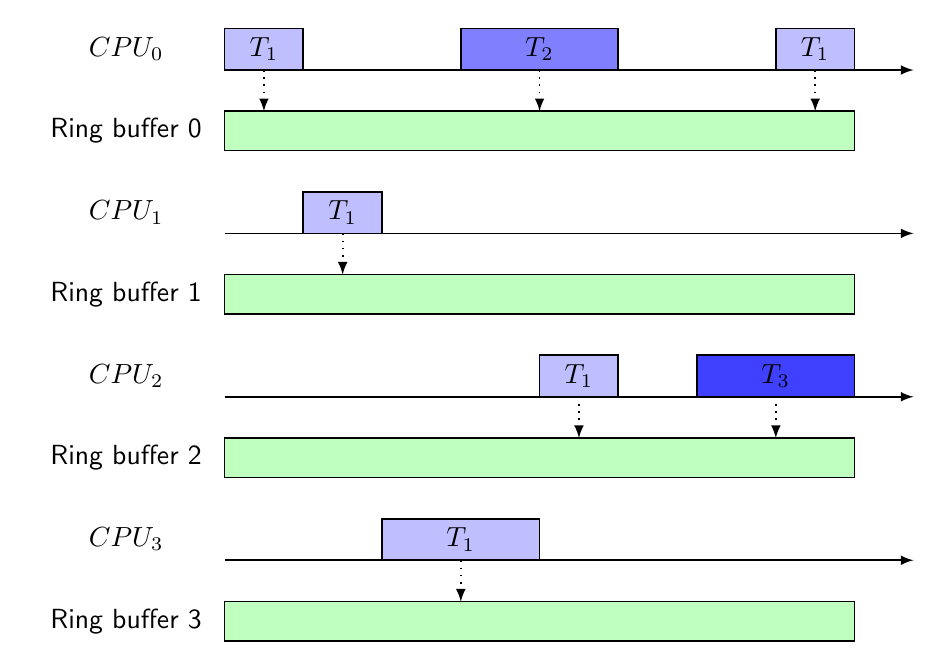
\begin{tikzpicture}[>=latex,font=\sffamily,semithick,scale=1.75]
	\node [minimum width=2.5cm,minimum height=.5cm,outer sep=0pt] at (0,0) (cpu0) {\( CPU_0 \)};
	\node [minimum width=1cm,minimum height=.5cm,outer sep=0pt,draw=black,fill=blue!25,right=0cm of cpu0] at (cpu0.east) (cpu0_p1_0) {\(T_{1}\)};
	\node [minimum width=2cm,minimum height=.5cm,outer sep=0pt,draw=black,fill=blue!50,right=3cm of cpu0] at (cpu0.east) (cpu0_p2_0) {\(T_{2}\)};
	\node [minimum width=1cm,minimum height=.5cm,outer sep=0pt,draw=black,fill=blue!25,right=7cm of cpu0] (cpu0_p1_1) {\(T_{1}\)};
	\draw[->] (cpu0.south east) -- +(5cm,0);

	\node [minimum width=2.5cm,minimum height=.5cm,outer sep=0pt,below=.5cm of cpu0] (rb0_txt) {Ring buffer 0};
	\node [minimum width=8cm,minimum height=.5cm,outer sep=0pt,draw=black,fill=green!25,right=0cm of rb0_txt] (rb0) {};

	\node [minimum width=2.5cm,minimum height=.5cm,outer sep=0pt,below=.5cm of rb0_txt] (cpu1) {\(CPU_{1}\)};
	\node [minimum width=1cm,minimum height=.5cm,outer sep=0pt,draw=black,fill=blue!25,right=1cm of cpu1] at (cpu1.east) (cpu1_p1_0) {\(T_{1}\)};
	\draw[->] (cpu1.south east) -- +(5cm,0);

	\node [minimum width=2.5cm,minimum height=.5cm,outer sep=0pt,below=.5cm of cpu1] (rb1_txt) {Ring buffer 1};
	\node [minimum width=8cm,minimum height=.5cm,outer sep=0pt,draw=black,fill=green!25,right=0cm of rb1_txt] (rb1) {};

	\node [minimum width=2.5cm,minimum height=.5cm,outer sep=0pt,below=.5cm of rb1_txt] (cpu2) {\(CPU_{2}\)};
	\node [minimum width=1cm,minimum height=.5cm,outer sep=0pt,draw=black,fill=blue!25,right=4cm of cpu2] (cpu2_p1_0) {\(T_{1}\)};
	\node [minimum width=2cm,minimum height=.5cm,outer sep=0pt,draw=black,fill=blue!75,right=6cm of cpu2] (cpu2_p3_0) {\(T_{3}\)};
	\draw[->] (cpu2.south east) -- +(5cm,0);

	\node [minimum width=2.5cm,minimum height=.5cm,outer sep=0pt,below=.5cm of cpu2] (rb2_txt) {Ring buffer 2};
	\node [minimum width=8cm,minimum height=.5cm,outer sep=0pt,draw=black,fill=green!25,right=0cm of rb2_txt] (rb2) {};

	\node [minimum width=2.5cm,minimum height=.5cm,outer sep=0pt,below=.5cm of rb2_txt] (cpu3) {\(CPU_{3}\)};
	\node [minimum width=2cm,minimum height=.5cm,outer sep=0pt,draw=black,fill=blue!25,right=2cm of cpu3] (cpu3_p1_0) {\(T_{1}\)};
	\draw[->] (cpu3.south east) -- +(5cm,0);

	\node [minimum width=2.5cm,minimum height=.5cm,outer sep=0pt,below=.5cm of cpu3] (rb3_txt) {Ring buffer 3};
	\node [minimum width=8cm,minimum height=.5cm,outer sep=0pt,draw=black,fill=green!25,right=0cm of rb3_txt] (rb3) {};

	\draw[->,dotted] (cpu0_p1_0.south) -- (cpu0_p1_0.south|-rb0.north);
	\draw[->,dotted] (cpu0_p1_1.south) -- (cpu0_p1_1.south|-rb0.north);
	\draw[->,dotted] (cpu0_p2_0.south) -- (cpu0_p2_0.south|-rb0.north);

	\draw[->,dotted] (cpu1_p1_0.south) -- (cpu1_p1_0.south|-rb1.north);

	\draw[->,dotted] (cpu2_p1_0.south) -- (cpu2_p1_0.south|-rb2.north);
	\draw[->,dotted] (cpu2_p3_0.south) -- (cpu2_p3_0.south|-rb2.north);

	\draw[->,dotted] (cpu3_p1_0.south) -- (cpu3_p1_0.south|-rb3.north);
\end{tikzpicture}
\par
\textbf{Figure 5: Ring buffer for system wide mode}
\end{center}

\subsection*{Writing and reading buffer}

From the previous section we get to know how the ring buffer is allocated for different modes, based on that this section will explain how the ring buffer is written or read.

\subsubsection*{Producer-consumer model}

It's a typical producer-consumer model for using the ring buffer.  In the Linux kernel, the events can produce samples which are stored into the ring buffer; the perf in user space consumes the samples by reading out the data from the ring buffer.

There have many occasions for generating samples: PMU interrupt handler when detecting event overflow, scheduling, dynamic tracepoint with kprobe/uprobe, static tracepoint, etc.  When a sample is recorded into the ring buffer, the kernel event core layer will wake up the thread which is polling on the events; perf works as a process to poll on the event, it will be waken up to read samples from the ring buffer.

\begin{center}
\par
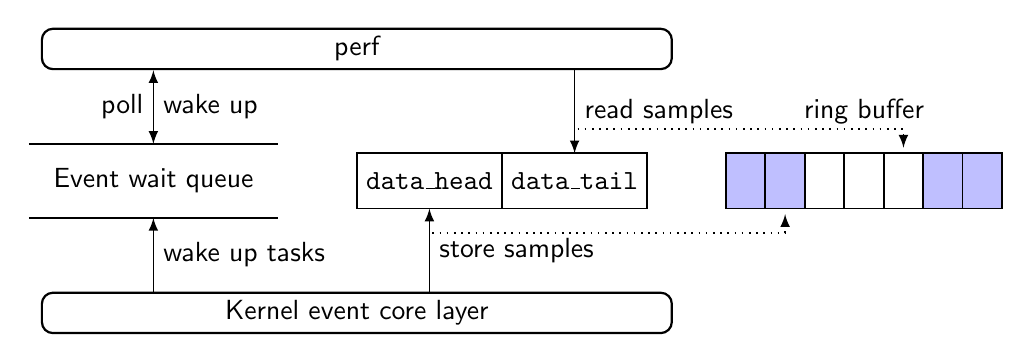
\begin{tikzpicture}[>=latex,font=\sffamily,semithick,scale=1.75]
	\node [minimum width=1cm,minimum height=2em,outer sep=0pt,draw=black,fill=white] at (0,0) (A) {\code{data\_head}};
	\node [minimum height=2em] at (A.east) (A2) {};
	\node [minimum width=1cm,minimum height=2em,outer sep=0pt,draw=black,fill=white,anchor=west] at (A.east) (B) {\code{data\_tail}};
        \node [minimum width=.5cm,minimum height=2em,outer sep=0pt,draw=black,fill=blue!25,right=1cm of B] (C) {};
        \node [minimum width=.5cm,minimum height=2em,outer sep=0pt,draw=black,fill=blue!25,anchor=west] at (C.east) (D) {};
        \node [minimum width=.5cm,minimum height=2em,outer sep=0pt,draw=black,fill=white,anchor=west] at (D.east) (E) {};
        \node [minimum width=.5cm,minimum height=2em,outer sep=0pt,draw=black,fill=white,anchor=west] at (E.east) (F) {};
        \node [minimum width=.5cm,minimum height=2em,outer sep=0pt,draw=black,fill=white,anchor=west] at (F.east) (G) {};
        \node [minimum width=.5cm,minimum height=2em,outer sep=0pt,draw=black,fill=blue!25,anchor=west] at (G.east) (H) {};
        \node [minimum width=.5cm,minimum height=2em,outer sep=0pt,draw=black,fill=blue!25,anchor=west] at (H.east) (I) {};
	\node [minimum width=.5cm,minimum height=2em,outer sep=0pt,above=0.5em of F] (buffer) {ring buffer};

	\node [minimum width=8cm,draw,thick,rounded corners,inner sep=.1cm,below=4em of A.west] (kernel) {Kernel event core layer};

	\node [minimum width=8cm,draw,thick,rounded corners,inner sep=.1cm,above=4em of A.west] (perf) {perf};

	\node [draw,thick,shape=datastore,inner sep=.3cm,left=1cm of A.west] (wq) {Event wait queue};

	\draw [->,dotted,shorten >=2pt,shorten <=2pt,semithick] (A.south) -- +(0em,-.5em) -| (D.south);
	\draw [->,dotted,shorten >=2pt,shorten <=2pt,semithick] (B.north) -- +(0em,.5em) -| (G.north);
	\draw [->] (A.south|-kernel.north) -- node[midway,right] {store samples} (A.south);
	\draw [->] (B.north|-perf.south) -- node[midway,right] {read samples} (B.north);
	\draw [->] (wq.south|-kernel.north) -- node[midway,right] {wake up tasks} (wq.south);
  	\draw [<->] (wq.north|-perf.south) -- node[midway,left] {poll} node[midway,right] {wake up} (wq.north);
\end{tikzpicture}
\par
\textbf{Figure 6: Writing and reading the ring buffer}
\end{center}

Note, perf sleeps on the wait queue of the events rather than wait on the ring buffer; the ring buffer itself doesn't provide wait queue.  But the event core layer in kernel is not only to wake up the sleeping tasks based on the event, on the other hand, it wakes up tasks based on the whole ring buffer.

Because multiple events share the same ring buffer for recording samples, when any event sample is stored into the ring buffer, the kernel event core layer simply wakes up sleeping tasks relevant to the ring buffer.  This is fulfilled by the kernel function \code{ring\_buffer\_wakeup()} which iterates every event associated to the ring buffer and wakes up tasks on the wait queue of the events.

\begin{lstlisting}
static void ring_buffer_wakeup(struct perf_event *event)
{
	struct perf_buffer *rb;

	rcu_read_lock();
	rb = rcu_dereference(event->rb);
	if (rb) {
		list_for_each_entry_rcu(event, &rb->event_list, rb_entry)
			wake_up_all(&event->waitq);
	}
	rcu_read_unlock();
}
\end{lstlisting}

Perf works as a standalone process; and after its process is waken up, it starts to check the ring buffers one by one, if finds any ring buffer contains samples it will read out the samples for statistics.

We can get to know that the perf process is possible to run on any CPUs, this leads to the ring buffer can be accessed from multiple CPUs simultaneously, which causes race conditions and should be handled properly.  The details for handling race condition will be depicted later.

\subsubsection*{Writing samples into buffer}

When an event couter is overflow, a sample will be taken and saved into the ring buffer; the function \code{\_\_perf\_event\_output()} is used to fill samples into the ring buffer.

\begin{lstlisting}[escapechar = !]
static __always_inline int
__perf_event_output(struct perf_event *event,
                    struct perf_sample_data *data,
                    struct pt_regs *regs,
                    int (*output_begin)(struct perf_output_handle *,
                                        struct perf_sample_data *,
                                        struct perf_event *,
                                        unsigned int))
{
        struct perf_output_handle handle;
        struct perf_event_header header;
        int err;

        /* protect the callchain buffers */
        rcu_read_lock();

        perf_prepare_sample(&header, data, event, regs);

        err = output_begin(&handle, data, event, header.size);
        if (err)
                goto exit;

        perf_output_sample(&handle, &header, data, event);

        perf_output_end(&handle);

exit:
        rcu_read_unlock();
        return err;
}
\end{lstlisting}

These main functions are called for outputting a sample:
\begin{itemize}
	\item As its name indicates, the function \code{perf\_prepare\_sample()} prepares sample fields based on the sample type;
	\item \code{output\_begin()} is a function pointer, it's passed dynamically via the argument for different writing direction, its purpose is to prepare the info for writing ring buffer, when return back the ring buffer info is stored in structure \code{perf\_output\_handle};
	\item \code{perf\_output\_sample()} outputs the sample fields into the ring buffer;
	\item \code{perf\_output\_end()} updates the head pointer for user page so perf tool can see the latest value.
\end{itemize}

Let's look into \code{output\_begin()}.  Since the ring buffer supports two directions for writing: backward or forward, thus this function pointer is assigned according to the buffer's writing type, it can be \code{perf\_output\_begin\_forward()} or \code{...\_backward()} variant.

For the backward ring buffer due to the user page is mapped without \code{'PROT\_WRITE'}, the tool in user space has no chance to update tail pointer, therefore, this case uses only head pointer and doesn't use the tail pointer.  For the backward ring buffer, the head pointer points to the start of a sample, perf tool can read out the samples one by one based on sample's event size.

Alternatively, the forward ring buffer uses both head pointer and tail pointer for the buffer management, which is more often used in perf tool and matches the description in the section "Basic algorithm".  To simplify the description, below uses the forward type of ring buffer to explain how to write samples.

\begin{center}
\par
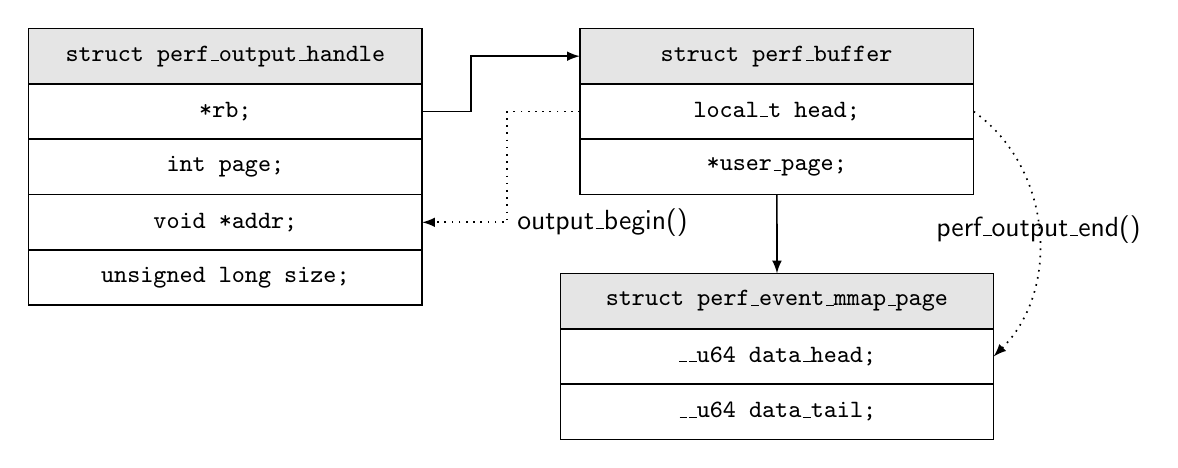
\begin{tikzpicture}[>=latex,font=\sffamily,semithick,scale=1.75]
	\node [minimum width=5cm,minimum height=2em,outer sep=0pt,draw=black,fill=gray!20] at (0,0) (oh) {\code{\small struct perf\_output\_handle}};
	\node [minimum width=5cm,minimum height=2em,outer sep=0pt,draw=black,fill=white,below=0cm of oh] (oh_rb) {\code{\small *rb;}};
	\node [minimum width=5cm,minimum height=2em,outer sep=0pt,draw=black,fill=white,below=0cm of oh_rb] (oh_page) {\code{\small int page;}};
	\node [minimum width=5cm,minimum height=2em,outer sep=0pt,draw=black,fill=white,below=0cm of oh_page] (oh_addr) {\code{\small void *addr;}};
	\node [minimum width=5cm,minimum height=2em,outer sep=0pt,draw=black,fill=white,below=0cm of oh_addr] (oh_size) {\code{\small unsigned long size;}};

	\node [minimum width=5cm,minimum height=2em,outer sep=0pt,draw=black,fill=gray!20,right=2cm of oh.east] (buf) {\code{\small struct perf\_buffer}};
	\node [minimum width=5cm,minimum height=2em,outer sep=0pt,draw=black,fill=white,below=0cm of buf] (buf_head) {\code{\small local\_t head;}};
	\node [minimum width=5cm,minimum height=2em,outer sep=0pt,draw=black,fill=white,below=0cm of buf_head] (buf_user_page) {\code{\small *user\_page;}};

	\node [minimum width=5.5cm,minimum height=2em,outer sep=0pt,draw=black,fill=gray!20,below=1cm of buf_user_page] (up) {\code{\small struct perf\_event\_mmap\_page}};
	\node [minimum width=5.5cm,minimum height=2em,outer sep=0pt,draw=black,fill=white,below=0cm of up] (up_head) {\code{\small \_\_u64 data\_head;}};
	\node [minimum width=5.5cm,minimum height=2em,outer sep=0pt,draw=black,fill=white,below=0cm of up_head] (up_tail) {\code{\small \_\_u64 data\_tail;}};

	\draw [->,semithick] (oh_rb.east) -- +(1em,0em) |- (buf.west);
	\draw [->,semithick] (buf_user_page.south) -- (up.north);
	\draw[->,dotted] (buf_head.east) to[bend left=50] node[midway] {perf\_output\_end()} (up_head.east);
	\draw[->,dotted] (buf_head.west) -- +(-1.5em,0em) |- node[midway,right] {output\_begin()} (oh_addr.east);
\end{tikzpicture}
\par
\textbf{Figure 7: Structures for writing ring buffer}
\end{center}

The event core layer in kernel uses the structure \code{perf\_buffer} to track the buffer's latest header, and it keeps the information for buffer pages.  If considering the life cycle, the structure \code{perf\_buffer} is allocated once the ring buffer is created, and it's released when the ring buffer is destroyed.

It's possible that multiple events to write buffer concurrently.  For instance, one software event and one hardware PMU event both are enabled for profiling, when the software event is in the middle of sampling, the hardware event maybe overflow and its interrupt is triggered in this case.  This leads to the race condition for \code{perf\_buffer::head}, because the software event sampling can be interrupted by the hardware event sampling.

Linux kernel uses compare-and-swap atomicity \code{local\_cmpxchg()} to implement the locklesss mechanism for protecting \code{perf\_buffer::head} (copied from \code{\_\_perf\_output\_begin()}):

\begin{lstlisting}
do {
        tail = READ_ONCE(rb->user_page->data_tail);
        offset = head = local_read(&rb->head);
        if (!rb->overwrite) {
                if (unlikely(!ring_buffer_has_space(head, tail,
                                                    perf_data_size(rb),
                                                    size, backward)))
                        goto fail;
        }

        /*
         * The above forms a control dependency barrier separating the
         * @tail load above from the data stores below. Since the @tail
         * load is required to compute the branch to fail below.
         *
         * A, matches D; the full memory barrier userspace SHOULD issue
         * after reading the data and before storing the new tail
         * position.
         *
         * See perf_output_put_handle().
         */

        if (!backward)
                head += size;
        else
                head -= size;
} while (local_cmpxchg(&rb->head, offset, head) != offset);
\end{lstlisting}

Comparing to \code{perf\_buffer}, the structure \code{perf\_output\_handle} is only used during the event sampling.  When an event is overflow, it firstly uses the structure \code{perf\_output\_handle} to establish a context for buffer's accessing, afterwards, sampling only uses the field \code{perf\_output\_handle::addr} as the destination address for copying sample data. 

A significant benefit from the structure \code{perf\_output\_handle} is it allows different events to write buffer concurrently.  The stucture \code{perf\_output\_handle} maintains two contexts for the software event and hardware event separately, thus every event reserves its own memory space in the function \code{out\_begin()} and \code{perf\_output\_handle::addr} is used for filling samples.

Until the sample data has been stored into buffer, the ring buffer's header is synced from \code{perf\_buffer::head} to \code{perf\_event\_mmap\_page::data\_head} in the function \code{perf\_output\_end()}.  This delivers the message to the perf tool that "now you are safe to read out the new samples from the user space".

\subsubsection*{Reading samples from buffer}

Like kernel's \code{perf\_output\_handle}, the structure \code{perf\_mmap} maintains a context for ring buffer in the user space, the context contains the info for buffer's start address, end address and mask; these values can be used to calculate the buffer pointer and size to be read based on different buffer modes.

The pointers and buffer are different data objects, it's possible for out-of-order accessing to them on the modern CPUs with relaxed memory model.  Furthermore, given perf and the profiled program running in multi-threads on multiple CPUs, the sequence between accessing pointers and buffer data must be promised by memory synchronization.

Besides the kernel function \code{perf\_output\_put\_handle()}, two helpers\\\code{ring\_buffer\_read\_head()} and \code{ring\_buffer\_write\_tail()} are introduced with memory barriers in the user space, they cooperates to ensure the data dependency; the rationale for the memory synchronization is:

\begin{tabular}{|l|l|}
\begin{minipage}{.4\textwidth}
\begin{lstlisting}[
tabsize=2,
numbersep=8pt,
numbers=left,
xleftmargin=0.5cm,frame=tlbr,framesep=2pt,framerule=0pt,
morekeywords ={class,run}
]
Kernel

if (LOAD ->data_tail) {
                   (A)
   STORE $data
   smp_wmb()       (B)
   STORE ->data_head
}
\end{lstlisting}
\end{minipage}

&

\begin{minipage}{.4\textwidth}
\begin{lstlisting}[
tabsize=2,
numbersep=8pt,
numbers=left,
xleftmargin=0.5cm,frame=tlbr,framesep=2pt,framerule=0pt,
aboveskip=-1.4\medskipamount,
morekeywords ={class,run}
]
User space

LOAD ->data_head
smp_rmb()       (C)
LOAD $data
smp_mb()        (D)
STORE ->data_tail
\end{lstlisting}
\end{minipage}
\end{tabular}

The comment in source file \code{include/linux/ring\_buffer.h} gives very nice description, here just tried to give explaination in my own words.

\code{(A)} indicates a control dependency between checking pointer \code{data\_tail} and filling sample, so that the kernel has chance to decide if the buffer has enough free space or not.  \code{(D)} needs to separate the ring buffer data reading from writing the pointer \code{data\_tail}, perf tool firstly reads samples and then tells kernel that samples have been consumed and it can safely use it from then on.  Since one of these two operations is reading and another is writing, thus it needs a full memory barrier.  \code{(B)} is a writing barrier in the middle of two writing operations, which makes sure the head pointer updating must be later than finishing current sampling.  \code{(C)} is a read memory barrier to split two read operations, it promises the program sequence for fetching the latest head pointer prior to reading samples.

Some architectures support one-way permeable barrier, such like load-acquire and store-release barriers are more relax to impose the barrier on any irrelevant memory operations, so \code{(C)} and \code{(D)} can be optimized to use barriers \code{smp\_load\_acquire()} and \code{smp\_store\_release()} respectively.

\begin{lstlisting}
static inline u64 ring_buffer_read_head(struct perf_event_mmap_page *base)
{
/*
 * Architectures where smp_load_acquire() does not fallback to
 * READ_ONCE() + smp_mb() pair.
 */
#if defined(__x86_64__) || defined(__aarch64__) || defined(__powerpc64__) || \
    defined(__ia64__) || defined(__sparc__) && defined(__arch64__)
        return smp_load_acquire(&base->data_head);
#else
        u64 head = READ_ONCE(base->data_head);

        smp_rmb();
        return head;
#endif
}

static inline void ring_buffer_write_tail(struct perf_event_mmap_page *base,
                                          u64 tail)
{
        smp_store_release(&base->data_tail, tail);
}
\end{lstlisting}

\end{document}
